\documentclass[landscape,24pt, a0paper,colspace=10mm,blockverticalspace=12mm]{tikzposter}

% Bibliography
\usepackage[backend=bibtex,firstinits=true,sorting=none, doi=false,isbn=false,url=false]{biblatex}
% Bibliography
%\bibliographystyle{unsrt}
\bibliography{Mendeley.bib}
\renewbibmacro{in:}{}
%\DeclareFieldFormat*{citetitle}{#1}
%\citefield{my-referenc}{title}
\DeclareFieldFormat*{title}{#1} 

%Remove 'references' title from bibliography
\usepackage{etoolbox}
\patchcmd{\thebibliography}{\section*{\refname}}{}{}{}

\usepackage{calculator}%For doing arithmetic?
\usepackage{verbatim}

\usepackage{amssymb, amsmath, mathrsfs, bm, mathtools}
\usepackage[makeroom]{cancel}

\newcommand{\Rm}{Rm}
\newcommand{\Da}{Da}
\newcommand{\Reynolds}{Re}
\newcommand{\Prandtl}{Pr}
\newcommand{\Ra}{Ra}

\newcommand{\St}{\mathscr{S}}
\newcommand{\ConcRatio}{\mathscr{C}}
\newcommand{\Le}{Le}


\newcommand*{\enthalpy}{\mathscr{H}}
\newcommand*{\RaT}{\ensuremath{Ra_T}}
\newcommand*{\RaTC}{\ensuremath{Ra_T^c}} %Critical rayleigh number
\newcommand*{\RaC}{\ensuremath{Ra_C}}
\newcommand*{\RaS}{\ensuremath{Ra_S}}
\newcommand*{\RmC}{\ensuremath{Rm_C}}
\newcommand*{\RmS}{\ensuremath{Rm_S}}
\newcommand*{\RmT}{\ensuremath{Rm_T}}
\newcommand*{\RmCrit}{\ensuremath{Rm_{crit}}}

\newcommand*{\Rmush}{\ensuremath{Rm}}
\newcommand*{\RaLiquid}{\ensuremath{Ra}}

\newcommand*{\RaCrit}{\ensuremath{Ra_c}}

\newcommand*{\Nu}{\ensuremath{Nu}}


\DeclareMathOperator\arctanh{arctanh}



% For displaying equations in tables
\usepackage{array}
%\def\tabularxcolumn#1{m{#1}} %ensure vertical centering
\newcolumntype{L}[1]{>{\raggedright\let\newline\\\arraybackslash\hspace{0pt}}m{#1}}
\newcolumntype{C}[1]{>{\centering\let\newline\\\arraybackslash\hspace{0pt}}m{#1}}
\newcolumntype{R}[1]{>{\raggedleft\let\newline\\\arraybackslash\hspace{0pt}}m{#1}}


 
\usepackage{authblk} %Formatting of author lists
\usepackage{enumitem} % For different itemize icons
\usepackage{graphicx,subcaption} % For subfigures
\usepackage{xcolor} %For colors in equations

%\definecolor{oxfordblue}{rgb}{0.0, 0.13, 0.28}
\definecolor{darkolivegreen}{rgb}{0.33, 0.42, 0.18}
\definecolor{darkmidnightblue}{rgb}{0.0, 0.2, 0.4}
\definecolor{darkpowderblue}{rgb}{0.0, 0.2, 0.6}
\definecolor{dodgerblue}{rgb}{0.12, 0.56, 1.0}
\definecolor{egyptianblue}{rgb}{0.06, 0.2, 0.65}
\definecolor{dukeblue}{rgb}{0.0, 0.0, 0.61}
\definecolor{falured}{rgb}{0.5, 0.09, 0.09}
\definecolor{royalfuchsia}{rgb}{0.79, 0.17, 0.57}

\newcommand{\varColor}[1]{\textcolor{dukeblue}{#1}}
\newcommand{\eqnColor}[1]{\textcolor{royalfuchsia}{#1}}
\newcommand{\paramColor}[1]{\textcolor{falured}{#1}}


\usepackage{pgfplots}
\usepgfplotslibrary{fillbetween}
\pgfplotsset{compat=1.13}

\usepackage{tikz}
\usetikzlibrary{calc,positioning,decorations.markings, backgrounds}

% Useful macro for finding out what the current font size is 
\makeatletter
\newcommand\thefontsize{{The current font size is: \f@size pt\par}}
\makeatother


\makeatletter

%24 pt for figure captions for AGU
\renewenvironment{tikzfigure}[1][]{
  \def \rememberparameter{#1}
  \vspace{10pt}
  \refstepcounter{figurecounter}
  \begin{center}
  }{
    \ifx\rememberparameter\@empty
    \else %nothing
    \\[24pt]
    {Fig.~\thefigurecounter: \rememberparameter}
    \fi
  \end{center}
}

% Title formatting
\def\TP@titlegraphictotitledistance{-4.5cm} % Without this, authors are below icons

\renewcommand\AB@affilsepx{, \protect\Affilfont}

\settitle{ \centering \vbox{

\centering
\vspace{-1.7cm}
\color{titlefgcolor} {\bfseries \Huge \sc \@title \par}
\vspace*{0.75cm} % Distance from title to graphics
% For title graphics. Uncomment next line to remove
\@titlegraphic \\ [\TP@titlegraphictotitledistance] 
{\LARGE \@author \par} \vspace*{1em} {\Large \@institute}
\vspace*{-5em}
}
}

\def\maketitle{\AB@maketitle} % prevent shifing content block to middle of page

\makeatother


%Define my block style
\defineblockstyle{MyBlock}{% define a custom style for a block
    titlewidthscale=1.0, bodywidthscale=1, titleleft,
    titleoffsetx=0pt, titleoffsety=0pt, bodyoffsetx=0pt, bodyoffsety=26mm,
    bodyverticalshift=16mm, roundedcorners=22, linewidth=5pt,
    titleinnersep=7mm, bodyinnersep=8mm
}{
    \draw[rounded corners=\blockroundedcorners, inner sep=\blockbodyinnersep,
          line width=\blocklinewidth, color=blocktitlefgcolor,
          top color=titlebgcolor, bottom color=titlebgcolor,
          fill=blockbodybgcolor
          ]
      (blockbody.south west) rectangle (blockbody.north east); %
}
\newcommand\myblock[3][MyBlock]{\useblockstyle{#1}\block{#2}{#3}\useblockstyle{Basic}}


% Theme details
\usetheme{Default} % See Section 5
\usebackgroundstyle{Empty}
\usetitlestyle[width=0.98\textwidth]{Default} 
\useblockstyle{MyBlock}

\definecolor{oxfordblue}{rgb}{0.0, 0.13, 0.28}

\definecolorstyle{sampleColorStyle} 
{
\definecolor{colorOne}{named}{blue}
\definecolor{colorTwo}{named}{yellow}
\definecolor{colorThree}{named}{orange} 
}{
% Background Colors
\colorlet{backgroundcolor}{white}
\colorlet{framecolor}{white}
% Title Colors
\colorlet{titlefgcolor}{oxfordblue}
\colorlet{titlebgcolor}{white} % white
% Block Colors
\colorlet{blocktitlebgcolor}{white} %oxfordblue
\colorlet{blocktitlefgcolor}{oxfordblue}
\colorlet{blockbodybgcolor}{oxfordblue} % white
\colorlet{blockbodyfgcolor}{black}
% Innerblock Colors
\colorlet{innerblocktitlebgcolor}{white}
\colorlet{innerblocktitlefgcolor}{black}
\colorlet{innerblockbodybgcolor}{colorThree!30!white}
\colorlet{innerblockbodyfgcolor}{black}
% Note colors
\colorlet{notefgcolor}{black}
\colorlet{notebgcolor}{colorTwo!50!white}
\colorlet{noteframecolor}{colorTwo}
}

\usecolorstyle[]{sampleColorStyle}


%Title text and graphics
\title{\parbox{\linewidth}{\centering Convection, phase change, and solute transport in mushy sea ice}} %with Adaptive Mesh Refinement
\titlegraphic{ \includegraphics[height=4cm]{figures/EGUSupplementaryContent.eps} 
\includegraphics[height=4cm]{figures/Oxford.eps}
\includegraphics[height=4cm]{figures/Berkeley_Lab_Logo_Small.eps} 
 \hfill 
  \includegraphics[height=4cm]{figures/nerc-logo.eps}  
     \includegraphics[height=4cm]{figures/roysoclogo.jpg} 
}
%For now title graphic:
%\titlegraphic{}

% Authors
\author[1]{James Parkinson (james.parkinson@physics.ox.ac.uk)}
\author[2]{Dan Martin}
\author[1]{Richard Katz}
\author[1]{Andrew Wells}
\affil[1]{University of Oxford}
\affil[2]{Lawrence Berkeley National Laboratory}



\tikzposterlatexaffectionproofoff % get rid of watermark in bottom right corner


 \tikzset{->-/.style={decoration={
  markings,
  mark=at position .5 with {\arrow[scale=2]{latex}}},postaction={decorate}}}


\begin{document}


\maketitle

\begin{columns} 

\column{0.21}

\block{Motivation}{

Sea ice is a mushy layer of ice crystals and brine. During ice formation, some of the dense brine drains into the ocean whilst some remains trapped in the ice.

Observations and 1D simulations suggest that atmospheric warming may enable drainage of remnant salt. \textbf{We investigate this mechanism using 2D simulations.}

} 


\block{What is a mushy layer?}
{
\vspace{-1cm}
\begin{tikzfigure}
\label{fig:phaseDiagram}
\begin{tikzpicture}

\node[anchor=north west] (fig2) at (0,0) {\includegraphics[width=0.4\linewidth, trim={0.0cm, 0.0cm, 0.0cm, 0.0cm}, clip]{figures/Eicken2000Edited.jpg} };

\node[anchor=north west] (phaseDiagram) at ([xshift=1.0cm]fig2.north east) {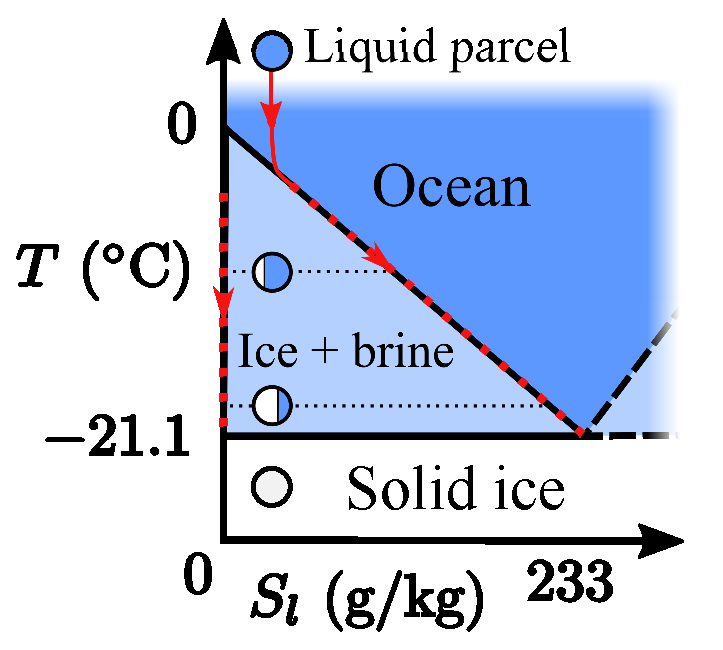
\includegraphics[width=0.47\linewidth, trim={0.0cm, 0.0cm, 0.0cm, 0.0cm}, clip]{figures/phaseDiagramVFinal.eps} };

\node[anchor=north west] (fig2label) at (fig2.north west) {(a)};

\node[anchor=north west] (fig1label) at ([yshift=0.0cm]phaseDiagram.north west) {(b)};

\end{tikzpicture}
\end{tikzfigure}
Fig. 2: (a)  Sea ice is a porous mixture of solid ice crystals (white) and liquid brine (dark) - image from Eicken et. al. (2000). (b) Trajectory ($\textcolor{red}{\rightarrow}$) of a solidifying salt water parcel through the $T-S_l$ phase diagram. As the temperature decreases, more ice forms whilst the residual brine becomes denser and can sink, triggering convection (see far right column).
}
\block{Numerical Method}
{
Solve (1)-(4) using Chombo finite volume toolkit:
\begin{itemize}
    \item Momentum and mass: projection method \cite{Martin2008}.
    \item Energy and solute:
    
%     \hspace{-\baselineskip}
%     \begin{minipage}[t]{8cm}
%     \textit{Advective terms:}  \\
%     explicit, 2\textsuperscript{nd} order unsplit Godunov.
%     \end{minipage} \hfill \vrule{} \hfill
%     \begin{minipage}[t]{12cm}
%     \textit{Nonlinear diffusive terms: } \\
%     semi implicit, geometric multigrid.
%     \end{minipage}

%    \item Timestepping: Backward Euler. 
     
   \begin{itemize}    
   \item Advective terms: explicit, 2\textsuperscript{nd} order unsplit Godunov method. %\cite{Colella1990}, 
   \item Nonlinear diffusive terms: semi implicit, geometric multigrid. %\cite{Martin1996}
   \item Timestepping: Backward Euler. %\cite{Twizell1996} 
   \end{itemize}
\end{itemize}
\vspace{-1ex}
}




\block[bodyoffsety=0mm, bodyverticalshift=0mm]{}{ %Need to specify some options to get rid of the title space
This work was funded by NERC and a travel grant from the Royal Society.
{
\fontsize{16}{15}\selectfont 
\renewcommand\refname{\vskip -2.5cm}
%\bibliography{bibliography}
\renewcommand*{\bibfont}{\scriptsize}
\printbibliography
}
\vspace{-0.75cm}
}

\column{0.55}

{ % start a group to keep the change of title background color local
\colorlet{blocktitlefgcolor}{red!60!black}
\colorlet{titlebgcolor}{red!5}
\block[bodyoffsety=0mm, bodyverticalshift=0mm]{}
{
\begin{minipage}[c]{12cm}
\vfill
\LARGE \textbf{Conclusions:}
\vfill
\end{minipage}\hfill
\begin{minipage}[c]{\linewidth - 12cm}
\Large 
\begin{itemize}
\item \textbf{... } 
\item \textbf{... }
\end{itemize}
\end{minipage}
}
}

\block{}{

\thefontsize

%Water of initial salinity $S_o=35\,\mathrm{g\,kg}^{-1}$ and temperature $-2^\circ$C is frozen from above in a Hele-Shaw cell with an open bottom boundary. A narrow plate separation $d=1$mm constrains the fluid flow everywhere, so (1) is well approximated by Darcy's law: $\mathbf{U} = \frac{K}{\eta} \left( - \nabla p + \rho_l \mathbf{g} \right)$. We assume $K_0=10^{-9}\,\mathrm{m}^2$, and consider different atmospheric temperatures $T_a$.
\begin{tikzfigure}
\begin{tikzpicture}
\node[anchor=north west, inner sep=0pt, outer sep=0pt] (BCs) at (0,0) {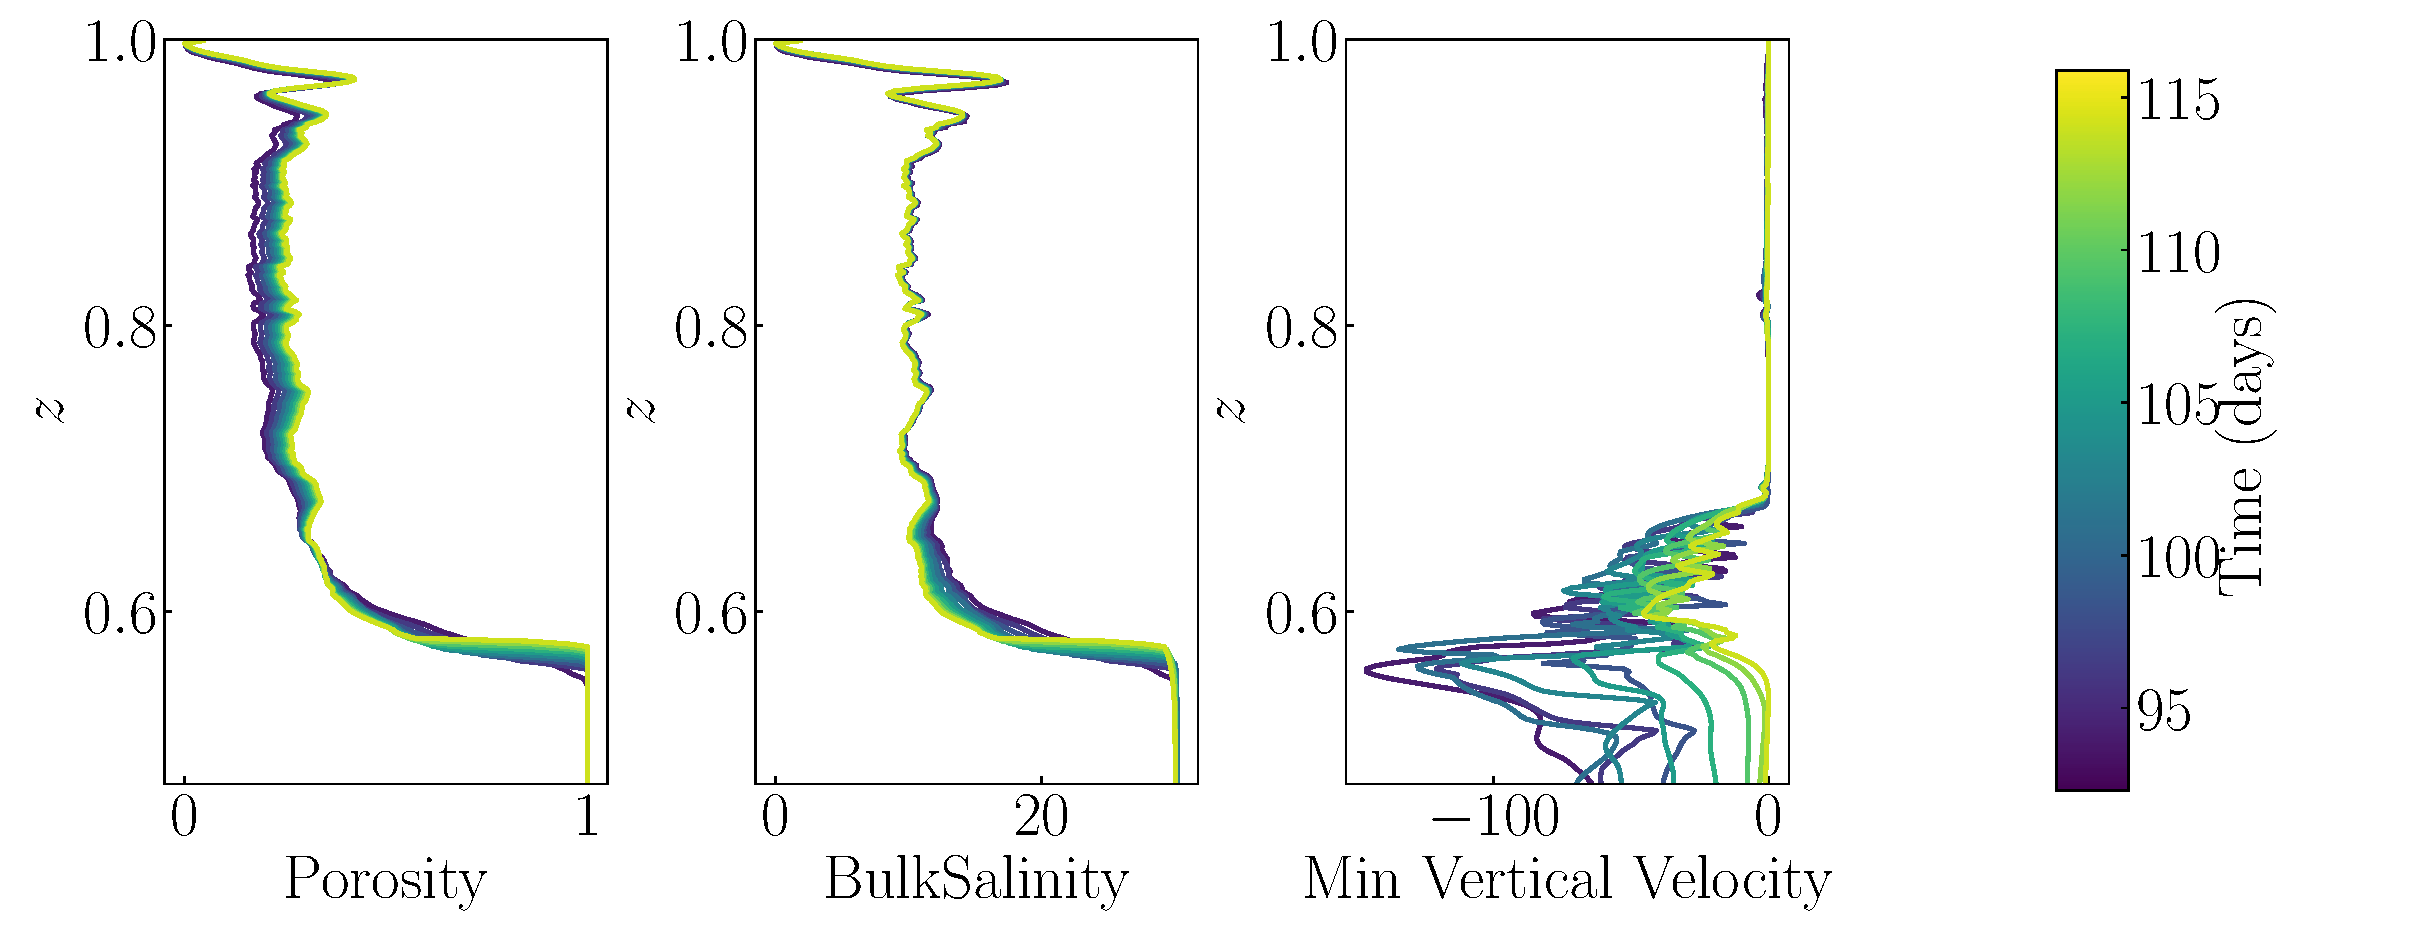
\includegraphics{figures/bottomMeltingProfiles.eps} };

%\node[anchor=south west, inner sep=0pt, outer sep=0pt] (aLabel) at ([xshift=-0.5cm, yshift=-0.8cm]BCs.north west) {(a)};

\end{tikzpicture}
\end{tikzfigure}

}

\block{Governing Equations for Flow in Porous Mushy Sea Ice in a Hele-Shaw cell}
{
Continuous equations for conservation of momentum (1), mass (2), salt~\eqref{eq:energy-cons} and energy~\eqref{eq:salt-cons} are found by averaging over lengths greater than the pore scale of sea ice \cite{Worster1991,LeBars2006}. \\
\begin{minipage}[t]{0.49\linewidth}

\begin{align}
\mathbf{U} = \frac{K(\chi)}{\eta} \left( \rho_l \mathbf{g} - \nabla p \right), \quad \quad   \nabla \cdot \mathbf{U} &= 0,   \tag*{(1, 2)}\label{eq:mom-mass} \\
    \frac{\partial S}{\partial t} + \mathbf{U} \cdot \nabla S_l &= \nabla \cdot \chi D_l \nabla S_l, \label{eq:salt-cons} \tag*{(3)} \\
    \frac{\partial H}{\partial t} + \rho_0 \, c_{p,l} \, \mathbf{U} \cdot \nabla  T &= \nabla \cdot \left[ k_l \chi + (1-\chi) k_s \right] \nabla T . \label{eq:energy-cons} \tag*{(4)}
\end{align} 
\end{minipage}
\hfill
\begin{minipage}[t][][b]{0.48\linewidth}
\vspace{-1.75\baselineskip}
\begin{align*}
&\varColor{\mathbf{U}}\; \text{(Darcy velocity)}, \quad \varColor{\chi} \; \text{(porosity)}, \quad \varColor{p} \; \text{(pressure)}, \quad \varColor{T} \; \text{(temperature)},\\
&\varColor{S_l} \; \text{(liquid salinity)}, \quad \varColor{S = \chi S_l} \; \text{(bulk salinity)},  \\
&\eqnColor{H = \rho_0 \left\{ L \chi + \left[\chi c_{p,l} + (1-\chi) c_{p,s}\right] T \right\}} \; \text{(enthalpy)}, \\
&\eqnColor{\rho_l = \rho_0 \left[1 - \alpha T + \beta S_l \right]} \; \text{(liquid density)}, \\
&\eqnColor{K(\chi)^{-1} = \left(d^2/12\right)^{-1} + \left[K_0 \chi^3 / (1-\chi)^2 \right]^{-1}} \; \text{(permeability)}, \\
&\paramColor{\eta} \; \text{(viscosity)}; \paramColor{D_l} \; \text{(salt diffusivity)}; \paramColor{\alpha}, \paramColor{\beta} \; \text{(thermal/haline expansion)}; \\
&\paramColor{c_{p,l}}, \paramColor{c_{p,s}} \; \text{(liquid/solid specific heat)}; \paramColor{k_l}, \paramColor{k_s} \; \text{(liquid/solid heat conductivity)}; \\
&\paramColor{d} \; \text{(Hele-Shaw cell thickness)}; \paramColor{K_0} \; \text{(Reference permeability)}.
\end{align*}
\end{minipage}



}

\column{0.245}

\block{Understanding salt fluxes}
{

}


\block{Future Work}
{
\begin{itemize}
%\item Investigation of salt fluxes from warming sea ice in the spring/summer.
%\item Investigate salt fluxes over longer time periods, and with time dependent atmospheric forcing.
%\item Simulations with a liquid region governed by eq (1), rather than flow in a Hele-Shaw cell.
%\item Simulations in three dimensions, including Adaptive Mesh Refinement.
\end{itemize}
}




\end{columns}

\end{document}
